% =========================================================
% Metric Spaces and Norms
% =========================================================

\subsection{Real Numbers as a Metric Space}

% =========================================================
\subsubsection{Basic Definitions}
% =========================================================

\begin{definition}[Modulus / Absolute value]
The \emph{modulus} (absolute value) is the function
\[
|\cdot| : \mathbb{R} \to \mathbb{R}
\]
defined by
\[
|x| :=
\begin{cases}
x, & x \ge 0,\\
-x, & x < 0.
\end{cases}
\]
\end{definition}

\begin{definition}[Distance function / Metric]
Let $X$ be a nonempty set. A function $d : X\times X \to \mathbb{R}$
is called a \emph{metric} on $X$ if for all $x,y,z\in X$:
\[
\begin{array}{rcl}
d(x,y) &\ge& 0, \\[0.35em]
d(x,y)=0 &\Longleftrightarrow& x=y, \\[0.35em]
d(x,y) &=& d(y,x), \\[0.35em]
d(x,z) &\le& d(x,y)+d(y,z).
\end{array}
\]
The pair $(X,d)$ is called a \emph{metric space}.
\end{definition}

\begin{definition}[Euclidean norm on $\mathbb{R}^n$]
For $x=(x_1,\dots,x_n)\in\mathbb{R}^n$, the \emph{Euclidean norm} is defined by
\[
\|x\|_2 := \left(\sum_{i=1}^n x_i^2\right)^{1/2}.
\]
\end{definition}

\begin{definition}[$\ell^p$ metrics]
Let $1\le p < \infty$. For $x,y\in\mathbb{R}^n$, define
\[
d_p(x,y)
=
\left(\sum_{i=1}^n |x_i - y_i|^p\right)^{1/p}.
\]
For $p=\infty$, define
\[
d_\infty(x,y)
=
\max_{1\le i\le n} |x_i - y_i|.
\]
\end{definition}

\begin{remark}
Throughout these notes, $|\cdot|$ denotes absolute value on $\mathbb{R}$,
while $\|\cdot\|_2$ denotes the Euclidean norm on $\mathbb{R}^n$.
\end{remark}

% =========================================================
\subsubsection{Main Theorems}
% =========================================================

\begin{theorem}[Properties of the modulus]
For all $x,y\in\mathbb{R}$:
\[
\begin{array}{rcl}
|x| &\ge& 0, \\[0.35em]
|x| = 0 &\Longleftrightarrow& x=0, \\[0.35em]
|-x| &=& |x|, \\[0.35em]
|xy| &=& |x|\,|y|, \\[0.35em]
|x+y| &\le& |x|+|y|, \\[0.35em]
\bigl||x|-|y|\bigr| &\le& |x-y|, \\[0.35em]
-|x| &\le& x \le |x|.
\end{array}
\]
\end{theorem}

\begin{remark}
The triangle inequality is the key property that allows
$|\cdot|$ to induce a metric:
\[
d(x,y)=|x-y|.
\]
\end{remark}

% =========================================================
\subsubsection{Canonical Examples}
% =========================================================

\begin{example}[Discrete metric]
Let $X$ be any nonempty set. Define
\[
d(x,y) :=
\begin{cases}
0, & x=y,\\
1, & x\neq y.
\end{cases}
\]
Then $d$ is a metric on $X$.
\end{example}

\begin{example}[Taxicab (Manhattan) metric]
On $\mathbb{R}^n$, define
\[
d_1(x,y) := \sum_{i=1}^n |x_i - y_i|.
\]
\end{example}

\begin{example}[London railway metric]
Fix a base point $0\in\mathbb{R}^n$.
Define
\[
d_L(x,y) :=
\begin{cases}
\|x\|_2 + \|y\|_2, & x \neq y,\\
0, & x = y.
\end{cases}
\]
Then $d_L$ is a metric.
\end{example}

% =========================================================
\subsubsection{Consequences}
% =========================================================

\begin{remark}[Geometric dependence on metric]
Let $(\mathbb{R}^2,d)$ be equipped with a norm $\|\cdot\|$.
The unit sphere is
\[
S = \{ x \in \mathbb{R}^2 : \|x\| = 1 \}.
\]

Changing the norm changes the geometry:

\begin{itemize}
\item $\ell^2$ → circle
\item $\ell^1$ → diamond
\item $\ell^\infty$ → square
\item $1<p<\infty$ → smooth interpolation between diamond and square
\end{itemize}

Although geometry changes, the logical structure of convergence
in metric spaces depends only on the metric axioms.
\end{remark}

\begin{remark}[Logical Structure]
\[
\text{Absolute Value}
\Rightarrow
\text{Triangle Inequality}
\Rightarrow
\text{Metric}
\Rightarrow
\text{Open Balls}
\Rightarrow
\text{Convergence Definition}
\]
\end{remark}

% =========================================================
\subsubsection{Geometric Illustration}
% =========================================================

\begin{center}
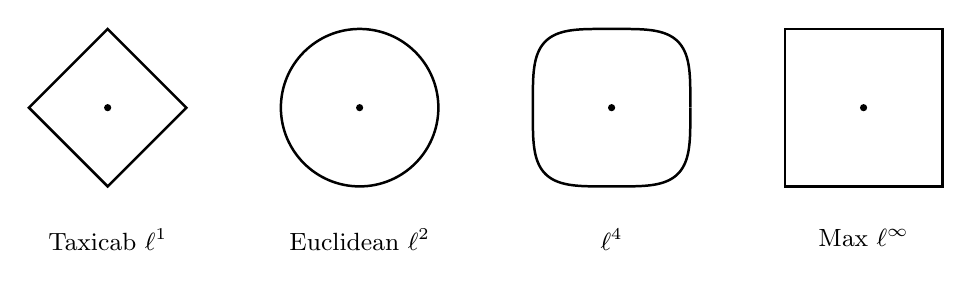
\begin{tikzpicture}[scale=1.0, line width=0.9pt]

\def\dx{3.2}
\def\s{1}

% L1
\begin{scope}[shift={(0,0)}]
  \draw (0,\s) -- (\s,0) -- (0,-\s) -- (-\s,0) -- cycle;
  \fill (0,0) circle (1.3pt);
  \node[below=6pt] at (0,-1.2) {\small Taxicab $\ell^1$};
\end{scope}

% L2
\begin{scope}[shift={(\dx,0)}]
  \draw (0,0) circle (\s);
  \fill (0,0) circle (1.3pt);
  \node[below=6pt] at (0,-1.2) {\small Euclidean $\ell^2$};
\end{scope}

% L4
\begin{scope}[shift={(2*\dx,0)}]
  \draw plot[domain=0:360,samples=200]
    ({\s*sign(cos(\x))*abs(cos(\x))^(1/2)},
     {\s*sign(sin(\x))*abs(sin(\x))^(1/2)});
  \fill (0,0) circle (1.3pt);
  \node[below=6pt] at (0,-1.2) {\small $\ell^4$};
\end{scope}

% L∞
\begin{scope}[shift={(3*\dx,0)}]
  \draw (-\s,-\s) rectangle (\s,\s);
  \fill (0,0) circle (1.3pt);
  \node[below=6pt] at (0,-1.2) {\small Max $\ell^\infty$};
\end{scope}

\end{tikzpicture}
\end{center}
